% This is "sig-alternate.tex" V2.1 April 2013
% This file should be compiled with V2.5 of "sig-alternate.cls" May 2012
%
% This example file demonstrates the use of the 'sig-alternate.cls'
% V2.5 LaTeX2e document class file. It is for those submitting
% articles to ACM Conference Proceedings WHO DO NOT WISH TO
% STRICTLY ADHERE TO THE SIGS (PUBS-BOARD-ENDORSED) STYLE.
% The 'sig-alternate.cls' file will produce a similar-looking,
% albeit, 'tighter' paper resulting in, invariably, fewer pages.
%
% ----------------------------------------------------------------------------------------------------------------
% This .tex file (and associated .cls V2.5) produces:
%       1) The Permission Statement
%       2) The Conference (location) Info information
%       3) The Copyright Line with ACM data
%       4) NO page numbers
%
% as against the acm_proc_article-sp.cls file which
% DOES NOT produce 1) thru' 3) above.
%
% Using 'sig-alternate.cls' you have control, however, from within
% the source .tex file, over both the CopyrightYear
% (defaulted to 200X) and the ACM Copyright Data
% (defaulted to X-XXXXX-XX-X/XX/XX).
% e.g.
% \CopyrightYear{2007} will cause 2007 to appear in the copyright line.
% \crdata{0-12345-67-8/90/12} will cause 0-12345-67-8/90/12 to appear in the copyright line.
%
% ---------------------------------------------------------------------------------------------------------------
% This .tex source is an example which *does* use
% the .bib file (from which the .bbl file % is produced).
% REMEMBER HOWEVER: After having produced the .bbl file,
% and prior to final submission, you *NEED* to 'insert'
% your .bbl file into your source .tex file so as to provide
% ONE 'self-contained' source file.
%
% ================= IF YOU HAVE QUESTIONS =======================
% Questions regarding the SIGS styles, SIGS policies and
% procedures, Conferences etc. should be sent to
% Adrienne Griscti (griscti@acm.org)
%
% Technical questions _only_ to
% Gerald Murray (murray@hq.acm.org)
% ===============================================================
%
% For tracking purposes - this is V2.0 - May 2012

\documentclass{sig-alternate-05-2015}


\begin{document}

% Copyright
\setcopyright{acmcopyright}
%\setcopyright{acmlicensed}
%\setcopyright{rightsretained}
%\setcopyright{usgov}
%\setcopyright{usgovmixed}
%\setcopyright{cagov}
%\setcopyright{cagovmixed}


% DOI
% \doi{10.475/123_4}

% ISBN
% \isbn{123-4567-24-567/08/06}

%Conference
% \conferenceinfo{PLDI '13}{June 16--19, 2013, Seattle, WA, USA}

% \acmPrice{\$15.00}

%
% --- Author Metadata here ---
% \conferenceinfo{WOODSTOCK}{'97 El Paso, Texas USA}
%\CopyrightYear{2007} % Allows default copyright year (20XX) to be over-ridden - IF NEED BE.
%\crdata{0-12345-67-8/90/01}  % Allows default copyright data (0-89791-88-6/97/05) to be over-ridden - IF NEED BE.
% --- End of Author Metadata ---

\title{Analog Sorting}
\subtitle{Theory and evaluation}
%
% You need the command \numberofauthors to handle the 'placement
% and alignment' of the authors beneath the title.
%
% For aesthetic reasons, we recommend 'three authors at a time'
% i.e. three 'name/affiliation blocks' be placed beneath the title.
%
% NOTE: You are NOT restricted in how many 'rows' of
% "name/affiliations" may appear. We just ask that you restrict
% the number of 'columns' to three.
%
% Because of the available 'opening page real-estate'
% we ask you to refrain from putting more than six authors
% (two rows with three columns) beneath the article title.
% More than six makes the first-page appear very cluttered indeed.
%
% Use the \alignauthor commands to handle the names
% and affiliations for an 'aesthetic maximum' of six authors.
% Add names, affiliations, addresses for
% the seventh etc. author(s) as the argument for the
% \additionalauthors command.
% These 'additional authors' will be output/set for you
% without further effort on your part as the last section in
% the body of your article BEFORE References or any Appendices.

\numberofauthors{2} %  in this sample file, there are a *total*
% of EIGHT authors. SIX appear on the 'first-page' (for formatting
% reasons) and the remaining two appear in the \additionalauthors section.
%
\author{
% You can go ahead and credit any number of authors here,
% e.g. one 'row of three' or two rows (consisting of one row of three
% and a second row of one, two or three).
%
% The command \alignauthor (no curly braces needed) should
% precede each author name, affiliation/snail-mail address and
% e-mail address. Additionally, tag each line of
% affiliation/address with \affaddr, and tag the
% e-mail address with \email.
%
% 1st. author
\alignauthor
Lusa Zhan\\
       \affaddr{Columbia University}\\
       \affaddr{Department of Computer Science}\\
       \affaddr{Department of Mathematics}\\
       \email{lz2371@columbia.edu}
% 2nd. author
\alignauthor
Yipeng Huang\\
       \affaddr{Columbia University}\\
       \affaddr{Department of Computer Science}\\
       \email{yipeng@cs.columbia.edu}
}
% There's nothing stopping you putting the seventh, eighth, etc.
% author on the opening page (as the 'third row') but we ask,
% for aesthetic reasons that you place these 'additional authors'
% in the \additional authors block, viz.
% \additionalauthors{Additional authors: John Smith (The Th{\o}rv{\"a}ld Group,
% email: {\texttt{jsmith@affiliation.org}}) and Julius P.~Kumquat
% (The Kumquat Consortium, email: {\texttt{jpkumquat@consortium.net}}).}
% \date{30 July 1999}
% Just remember to make sure that the TOTAL number of authors
% is the number that will appear on the first page PLUS the
% number that will appear in the \additionalauthors section.

\maketitle
\begin{abstract}
\end{abstract}


%
% The code below should be generated by the tool at
% http://dl.acm.org/ccs.cfm
% Please copy and paste the code instead of the example below. 
%
% \begin{CCSXML}
% <ccs2012>
%  <concept>
%   <concept_id>10010520.10010553.10010562</concept_id>
%   <concept_desc>Computer systems organization~Embedded systems</concept_desc>
%   <concept_significance>500</concept_significance>
%  </concept>
%  <concept>
%   <concept_id>10010520.10010575.10010755</concept_id>
%   <concept_desc>Computer systems organization~Redundancy</concept_desc>
%   <concept_significance>300</concept_significance>
%  </concept>
%  <concept>
%   <concept_id>10010520.10010553.10010554</concept_id>
%   <concept_desc>Computer systems organization~Robotics</concept_desc>
%   <concept_significance>100</concept_significance>
%  </concept>
%  <concept>
%   <concept_id>10003033.10003083.10003095</concept_id>
%   <concept_desc>Networks~Network reliability</concept_desc>
%   <concept_significance>100</concept_significance>
%  </concept>
% </ccs2012>  
% \end{CCSXML}

% \ccsdesc[500]{Computer systems organization~Embedded systems}
% \ccsdesc[300]{Computer systems organization~Redundancy}
% \ccsdesc{Computer systems organization~Robotics}
% \ccsdesc[100]{Networks~Network reliability}


%
% End generated code
%

%
%  Use this command to print the description
%
% \printccsdesc

% We no longer use \terms command
%\terms{Theory}

\keywords{linear algebra; ordinary differential equations; algorithms}

\section{Introduction}

\section{Background}
\subsection{Classical sorting algorithms}
While digital sorting algorithms are efficient, no prior work has discussed what the time complexity of analog sorting. To get a sense of how analog sorting performs, we need a basis for comparison. Some of the classical sorting algorithms are merge sort or quick sort. Those generally have nonlinear time complexity, but quick sort has logarithmic space complexity. Table 1 lists some algorithms and their respective complexities.

Later, we will analyze how analog sorting compares to digital sorting algorithms in terms of complexity. 

\begin{table}[h]
\centering
\caption{Complexities of Sorting Algorithms}
\begin{tabular}{|l|c|c|} \hline
Sorting Algorithm&Time Complexity&Space Complexity\\ \hline
Merge Sort & $O(n\log n)$& $O(n)$\\ \hline
Quick Sort & $O(n\log n)$& $O(\log n)$\\ \hline
Insertion Sort & $O(n^2)$& $O(1)$\\ \hline
Selection Sort & $O(n^2)$& $O(1)$\\
\hline\end{tabular}
\end{table}



% \begin{table*}
% \centering
% \caption{Some Typical Commands}
% \begin{tabular}{|c|c|l|} \hline
% Command&A Number&Comments\\ \hline
% \texttt{{\char'134}alignauthor} & 100& Author alignment\\ \hline
% \texttt{{\char'134}numberofauthors}& 200& Author enumeration\\ \hline
% \texttt{{\char'134}table}& 300 & For tables\\ \hline
% \texttt{{\char'134}table*}& 400& For wider tables\\ \hline\end{tabular}
% \end{table*}
% end the environment with {table*}, NOTE not {table}!
\subsection{The QR algorithm}
The analog sorting method we show is related to the classical QR algorithm.
While the QR algorithm is a discrete algorithm operating step-by-step, the analog sorting algorithm does so in continuous time~\cite{chu_realization, chu_flows, deift}.

The QR algorithm finds the eigenvalues and eigenvectors of a square matrix.
The eigenvalue problem is as follows:
\[A_0x = \lambda x\]

The QR algorithm operates as follows:
Given the QR decomposition, each step proceeds as:
\[A_k = Q_k R_k\]
\[A_{k+1} = R_k Q_k\]

A side effect of the QR algorithm is that the eigenvalues of the original matrix end up in sorted order along the diagonal.
This is a useful property in eigenvalue problems, where users of the algorithm are interested in finding the largest few eigenvalues.
But few researchers have pointed out that this may be useful in itself, for sorting.
Other algorithms for finding the eigenvalues and eigenvectors include the Jacobi eigenvalue algorithm, and the divide-and-conquer algorithm.
It seems that the QR algorithm is the algorithm among these that sorts the eigenvalues.

The close relationship between the analog sorting method and the QR algorithm implies that they should have similar properties as well.

\subsection{Hamiltonian systems}
\newcommand*{\hham}{\hat{\mathcal{H}}}
The finite Toda lattice system of ODEs belongs to special class of ODEs called Hamiltonian systems.
Hamiltonian systems are an important and efficient way to describe classical mechanics.
Because of their importance, special ODE solvers called symplectic solvers have been developed specifically to solve Hamiltonian systems.

A Hamiltonian system is characterized by a total energy scalar $\hham$.
The components of the system are described by vectors $p$ for momenta and $q$ for positions.
The system obeys the laws of motion:
\begin{align}
dp/dt &= -dH/dq = f(q)
dq/dt &= dH/dp = g(p)
\end{align}

% x and p encode what you want to sort
Conceptually, we encode the keys we like to sort as the momenta of particles.
The momenta of the particles carries them to a final state that represents the sorted system.
\subsection{Toda lattice, double bracket}
The finite Toda lattice is an ODE system that is related to the QR algorithm.
If you plot the evolution of the Toda lattice ODE with respect to time, the values of the ODE at integer time steps is the intermediate states of the QR algorithm.
% Bloch and Rojo: Section 3.2 of Bloch and Rojo paper says the Toda flow preserves the eigenvalues. This seems to be the main connection to the QR algorithm, which also preserves eigenvalues across iterations.
The common property of the finite Toda lattice and the QR algorithm is that both preserve the eigenvalues of the matrix they operate on~\cite{bloch}.

The finite Toda lattice is a Hamiltonian system with the form:
\begin{align}
\hham(p,q) = \frac{1}{2} \sum^{n}_{1}p_k^2 + \sum^{n-1}_{1}exp(q_k-q_{k+1})
\end{align}

This basic form can changed in two ways, using change of variables, into the equations for analog sorting described in~\cite{brockett}.

% \documentclass{article}
% \usepackage[utf8]{inputenc}
% \usepackage{amsmath}

% \title{Toda Lattice, Double Bracket}
% \author{Lusa Zhan}
% \date{September 2016}

% \begin{document}

% \maketitle


% \section{Equivalence between ODE and Lie bracket notation}

The central idea of analog sorting as described in~\cite{bloch, brockett} makes use of the Toda lattice. The system of Hamiltonian equations in (1) associated with the Hamiltonian in (2) gives us the following set of equations
\begin{align*}
\dot{p_k} &= \exp(q_{k-1}-q_{k})-\exp(q_{k}-q_{k+1}) \\
\dot{q_k} &= p_k
\end{align*}
where the boundary conditions are set so that $\exp(x_0-x_1)=\exp (x_n-x_{n+1})=0$.

This system is also analogous to the double bracket notation 
\begin{align}
\dot{H} = [H,[H,N]]
\end{align}

where the brackets stand for the Lie bracket $[A,B] = AB-BA$. The connection between the Hamiltonian system  and the double bracket notation of the Toda lattice will be discussed and outlined in the following sections.

\subsubsection{Toda lattice - ODE form}

The above system of ordinary differential equations can be transformed into the system described in~\cite{harvard_robo} using a change of variables.
\begin{align}
x_k &= -\frac{1}{2}p_k \nonumber \\
y_k &= \frac{1}{2}\exp(\frac{q_k-q_{k+1}}{2})
\end{align}

In that case, 
\begin{align*}
    \dot{x_k} &= -\frac{1}{2}\dot{p_k} \\
              &= -\frac{1}{2}(exp(q_{k-1}-q_{k})-exp(q_{k}-q_{k+1})) \\
              &= -\frac{1}{2}(4y^2_{k-1}-4y^2_k) \\
              &= 2y^2_k-2y^2_{k-1}
\end{align*}

and 
\begin{align*}
    \dot{y_k} &= \frac{1}{2}\exp(\frac{q_k-q_{k+1}}{2})\frac{\dot q_k-\dot q_{k+1}}{2} \\
              &= y_k\frac{p_k-p_{k+1}}{2} \\
              &= y_k(x_{k+1}-x_k) 
\end{align*}

Taking into account the boundary conditions $y_0=y_n=0$, we get the desired system of ODEs with
\begin{align}
    \dot{x_k} &= 2y^2_k-2y^2_{k-1} \nonumber \\
    \dot{y_k} &= y_k(x_{k+1}-x_k) \\
    y_0 &= y_n = 0 \nonumber
\end{align}

This is the system of ODEs we will solve in the analog chip and in our simulations.


\subsubsection{Toda lattice - Jacobi matrix}

The connection between the Toda lattice and the double bracket notation $\dot{H} = [H,[H,N]]$ can be made through the Jacobi Matrix form of the Toda lattice. The Jacobi matrix for the Hamiltonian system after the change of variables (4) is given by
\begin{align}
 H = \begin{bmatrix}
    x_{1} & y_{1} & 0  & \dots & 0 \\
    y_{1} & x_{2} & y_{2} & \dots & 0 \\
     & & \ddots & \\
          &       & y_{n-2} & x_{n-1} & y_{n-1}\\
    0 & \hdots & & y_{n-1} & x_{n}
\end{bmatrix}
\end{align}
This is the form of $H$ required for analog sorting as outlined by Brockett in ~\cite{brockett}.

In order to get the double bracket form, we need a diagonal matrix $N = \text{diag}(n, n-1, \dots, 1)$ whose role will be discussed in 2.5.1.

\begin{align*}
N = \begin{bmatrix}
        n & 0 & \hdots & 0 \\
        0 & n-1 & \\
        \vdots &  & \ddots & \vdots \\
        0 & \hdots & & 1
    \end{bmatrix}
\end{align*}

From this, we can calculate $[H[H,N]] = H[H,N]-[H,N]H$ step by step:

\[ 
HN = \begin{bmatrix}
        nx_1 & (n-1)y_1 & \hdots & 0 \\
        ny_1 & (n-1)x_2 & \hdots & 0 \\
        \vdots & & \ddots & 0\\
         &  & 2x_{n-1} & y_{n-1} \\
        0 & \hdots & 2y_{n-1} & x_n

    \end{bmatrix}
\]

\[ 
NH = \begin{bmatrix}
        nx_1 & ny_1 & \hdots & 0 \\
        (n-1)y_1 & (n-1)x_2 & \hdots & 0 \\
        \vdots & & \ddots & 0\\
         &  & 2x_{n-1} & 2y_{n-1} \\
        0 & \hdots & y_{n-1} & x_n

    \end{bmatrix}
\]

\[ 
HN-NH = \begin{bmatrix}
        0 & -y1 & \hdots &  & 0 \\
        y_1 & 0 & -y_2 & \hdots & 0 \\
        \vdots & \ddots & \ddots & \ddots & 0\\
         & & y_{n-2}& 0 & -y_{n-1} \\
        0 & & \hdots & y_{n-1} & 0

    \end{bmatrix}
\]

\[ 
H[H,N] = \begin{bmatrix}
        y_1^2 & -x_1y_1 & \hdots & 0 \\
        x_2y_1 & -y_1^2+y^2_2 &\hdots & 0 \\
        y_1y_2 & \ddots & & 0\\
        \vdots & & y^2_{n-1}-y^2_{n-2} & -x_{n-1}y_{n-1} \\
        0 & \hdots & x_ny_{n-1} & -y^2_{n-1}

    \end{bmatrix}
\]

\[ 
[H,N]H = \begin{bmatrix}
        y_1^2 & -x_2y_1 & \hdots & 0 \\
        x_1y_1 & y_1^2-y^2_2 &\hdots & 0 \\
        y_1y_2 & \ddots & & 0\\
        \vdots &  & -y^2_{n-1}+y^2_{n-2} & -x_{n}y_{n-1} \\
        0 & \hdots & x_{n-1}y_{n-1} & y^2_{n-1}

    \end{bmatrix}
\]
\\

Therefore, we get \\

\[[H,[H,N]] = 
\begin{bmatrix}
    2y_1^2 & y_1(x_2-x_1) & 0 \\
    y_1(x_2-x_1) & -2(y_1^2-y^2_2) & 0\\
    0 & \ddots & 0\\
    \vdots & & y_{n-1}(x_{n}-x_{n-1}) \\
    0 & \hdots & -2y^2_{n-1}
\end{bmatrix}
\]

This is equivalent to the result we get from combining the matrix form of $H$ with the values for $\dot{x}$ and $\dot{y}$
\[\dot{H} = \begin{bmatrix}
    \dot{x}_{1} & \dot{y}_{1} & 0  & \dots & 0 \\
    \dot{y}_{1} & \dot{x}_{2} & \dot{y}_{2} & \dots & 0 \\
     & & \ddots & \\
     & & \dot{y}_{n-2} & \dot{x}_{n-1} & \dot{y}_{n-1}\\
    0 & \hdots & & \dot{y}_{n-1} & \dot{x}_{n}
    
\end{bmatrix}\]

In total, we conclude that the double bracket notation of the Toda lattice used in other papers is analogous to the system of ODEs. We use the equivalent system of ODEs to construct the analog sorter.




%\documentclass{article}
%\usepackage[utf8]{inputenc}
%\usepackage{amsmath}

%\title{Toda Lattice, Role of $N$ and $y_k$}
%\author{Lusa Zhan}
%\date{November 2016}

%\begin{document}

%\maketitle

\subsubsection{Role of $N$}
The choice of $N = \text{diag} (n, n-1, \dots, 1)$ for analog sorting is clarified by Theorem 1.5 in~\cite{helmke}. To summarize, the theorem states the following: 

For each $N$,  $\dot{H}(t) = [H,[H,N]]$ converges to an equilibrium $H_\infty$ as $t\rightarrow \infty$. If $N=\text{diag} (\mu_1 , \dots , \mu_n)$ where $\mu_1 > \dots > \mu_n$, then the Hessian of $f_N(H) = \frac{1}{2}\|N-H\|^2$ is nonsingular and negative definite. 

The linearization of the double bracket flow at an equilibrium point $H_\infty = \text{diag}(\lambda_{\pi(1)},\dots,\lambda_{\pi(n)})$ is 
\[\dot \xi_{ij} = -(\lambda_{\pi(i)}-\lambda_{\pi(j)})(\mu_i-\mu_j)\xi_{ij}\]
where $\xi = [H_\infty, N]$. Since the Hessian is negative definite, $\xi$ must be at its maximum. If $N = \text{diag} (n, n-1, \dots, 1)$, then $\xi$ will only reach its maximum if the diagonal entries of $H_\infty$ are sorted in descending order as well.

Thus the diagonal matrix $N$ determines the order of the diagonal entries in $H_\infty$. Letting $N = \text{diag}(n, ,n-1, \dots, 1)$, we will result in $x_1 \geq x_2 \geq \cdots \geq x_n$ in $H_\infty$.

\subsubsection{Role of off-diagonals $y_k$}
The choice of initial values for the off-diagonal $y_k$ values affects the results of analog sorting as well. 

First of all, as mentioned previously, $y_0=y_n=0$.
To analyze the initial values of $y_k$, consider the relation to $\dot x_k$
\begin{align*}
    \dot{x_k} &=  2y^2_k-2y^2_{k-1} \\
    \dot{y_k} &= y_k(x_{k+1}-x_k) 
\end{align*}

If $y_k=0$, then $\dot x_k=0$, meaning $x_k(t) = x_k(0)$ for all $t$. This means that the values along the diagonal of $H$ will remain constant and never get sorted. So, $y_k$ should be non-zero.

In addition, the $y_k$ values should be small (but still positive). Recall that the eigenvalues will be the values along the diagonal of $H$ as $t\rightarrow \infty$. Consider the determinant $f_n = \det (H-\lambda I)$, where $n$ is the size of the matrix. Since $H$ is a tridiagonal matrix, this determinant can be formulated using a recurrence relation on the size of the matrix $n$.

\begin{align*}
f_n &= (x_n-\lambda)f_{n-1}-y_{n-1}^2f_{n-2} \\
f_1 &= x_1-\lambda
\end{align*}

We can use this to calculate the first few $f_n$ and set them to $0$ (what we would do to calculate the eigenvalues):
\begin{align*}
f_1 &= x_1-\lambda = 0\\
f_2 &= (x_2-\lambda)(x_1-\lambda)-y_1^2 = 0\\
f_3 &= (x_3-\lambda)(x_2-\lambda)(x_1-\lambda)-(x_3-\lambda)y_1^2-(x_1-\lambda)y^2_2 = 0
\end{align*}

Intuitively, the eigenvalues will be closest to $x_k$ if the $y_k$ values are smaller. When setting up the analog sorter, we want the off-diagonals to be nonzero, but small enough to not significantly change the values to be sorted. 



%\section{Related work}
%Below is a list of articles that are related to this topic: 
%\begin{itemize}

%\item{
%    Brockett, R.w. ``Dynamical Systems That Sort Lists, Diagonalize Matrices, and Solve Linear Programming Problems.'' Linear Algebra and Its Applications 146 (1991): 79-91. }
%\item{
%    Helmke, Uwe, and John B. Moore. ``Double Bracket Isospectral Flows.'' Optimization and Dynamical Systems. London: Springer-Verlag, 1994. 43-80. Print.}
%\end{itemize}


%\end{document}


% equivalently, the Toda flow is
% dX/dt = [X(t), pi_0(X(t))]
% =X(t) pi_0(X(t)) - pi_0(X(t)) X(t)

% where pi_0 = X^- - X^{-T}
% where X^- is the lower triangular part
\subsection{Realizing the analog sorter}
We validate the functionality of analog sorting using a prototype analog computer chip.
After reviewing the mathematics of analog sorting, we now discuss how the analog sorter is put in practice.

The analog sorter works as follows:
% We set up a vector x, consisting of real numbers in a jumbled order.
We construct matrix $H(t=0)$ with the real numbers we want to sort on the diagonal and some small values on the off-diagonals.
Naturally $H(t=0)$ has eigenvalues consisting of the same real numbers.
We set up a special ODE that involves the vector $x$, and another vector consisting of the natural numbers.
This vector of the natural numbers provides the ``discreteness'' for the algorithm.
Specifically, this ODE is the finite Toda lattice ODE, which preserves the eigenvalues of $H(t)$, while reordering the elements on the diagonal to the sorted sequence.
This solves this ODE on an analog computer.
The final steady state of the analog output would have the original elements of the vector $x$, but now in sorted order.
For example, the first integrator would have the lowest magnitude element of $x$.

% It's still unclear to me:
% 1. What's the role of the off-diagonal parts of the symmetric, tridiagonal H. Brockett tells us to put some small values there to kick off the algorithm.
% 2. What's the role of the matrix of the natural numbers N.
% The matrix N of the natural numbers happens to make [H,N] have the form B on page 37 of Bloch & Rojo.
% Now, we can say that matrix N is the way it is just to make the HN-NH have a special shape.

% But, on the other hand, N, being a matrix of integers, is the only participant in this system that has "discreteness." Otherwise the system is all real numbers evolving in continuous-time.

There are some variations to this idea.
One is we can tackle the finite Toda lattice system directly as a Hamiltonian system.
Another is we can reverse the roles of the sort keys and the indices.
This is described by Brockett briefly in page 802 of~\cite{brockett}.
% Way 1:
% H(0) is the tridiagonal, with the stuff we want to sort on the diagonal. Off diagonal, some small values. N is diagonal matrix of the natural numbers.
% Way 2:
% N is diagonal matrix of the stuff we want to sort.
% swapping two vars
% decreases the sparsity
% but this is important because this way you move the indexes, instead of keys

\section{Methodology}
We validate the functionality of analog sorting using a prototype analog computer chip.
In order to explore how analog sorting works in larger systems, we use an ODE solver built on the odeint solver in the Python SciPy library.

% The code here
% https://github.com/mandli/intro-numerical-methods/blob/master/09_ODE_ivp.ipynb
% Would be a good starting point for the simulation. 

% https://docs.scipy.org/doc/numpy/reference/generated/numpy.linalg.qr.html
% http://docs.scipy.org/doc/scipy/reference/generated/scipy.integrate.ode.html#scipy.integrate.ode
% http://docs.scipy.org/doc/scipy/reference/generated/scipy.integrate.odeint.html

\section{Evalution}
After testing analog sorting on a prototype analog computer chip and simulating the process using an ODE solver, we can evaluate its time and space complexity. 

Compared to the other sorting algorithms mentioned at the beginning of the paper, analog sorting performs better in terms of time complexity. However, due to the nature of circuits, it is not as space efficient as most other popular sorting algorithms.

\subsection{Functionality validation of analog sorting}

\begin{figure}[h]
\centering
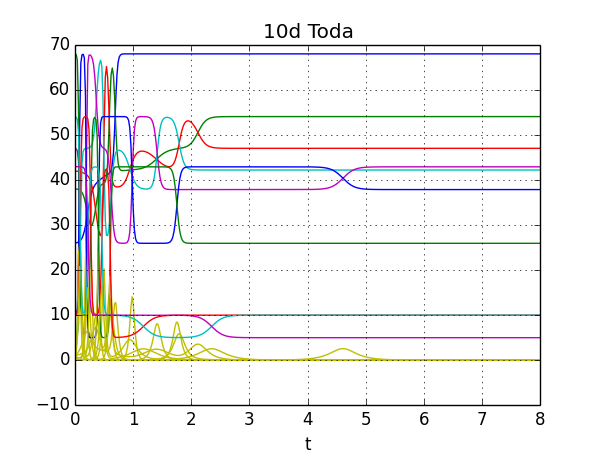
\includegraphics[width=\columnwidth]{graphics/10d_toda_7.png}
\caption{Simulated sorting a 10 element vector.}
\end{figure}

We see in Figure 1, generated from the ODE solver, that the sorting system has periods of swapping, interspersed in quiet periods of little change. The ODE solver was used on a 10 element vector. 

The output of the analog chip, run on two variables and over multiple loops, is shown in the below image.

\begin{figure}[h]
\centering
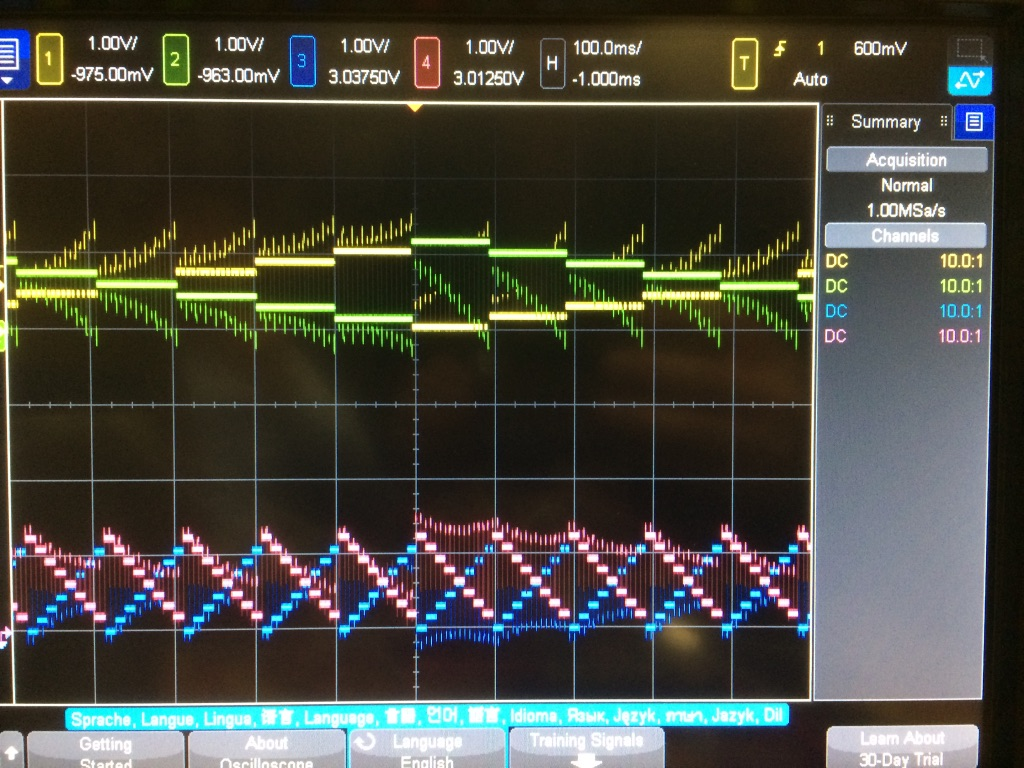
\includegraphics[width=\columnwidth]{graphics/2d_analog.jpg}
\caption{Sorted 2 elements using analog computer chip.}
\end{figure}

 

\subsection{Time cost of the discrete QR algorithm}
Time cost of overall QR loop:
	how many iterations of qr til convergence?
	% time to convergence of qr w.r.t.. problem size
	Since we know the ODE is analogous to QR algorithm, they should take the same amount of time.
Time cost of QR step:
	Numerical Recipes 3rd Edition p585 says the QR algorithm takes $O(N)$ time for symmetric tridiagonal matrices.

\subsection{Time cost of analog sorting}

In terms of time, the sorter takes at least $O(N)$ time because of the time it takes just for signals to propagate across the circuit.
Another issue is the time it takes for the ODE to settle to its final value.
This shows preliminary data showing the time to convergence of analog sorting, plotted against problem size.

\begin{figure}[h]
\centering
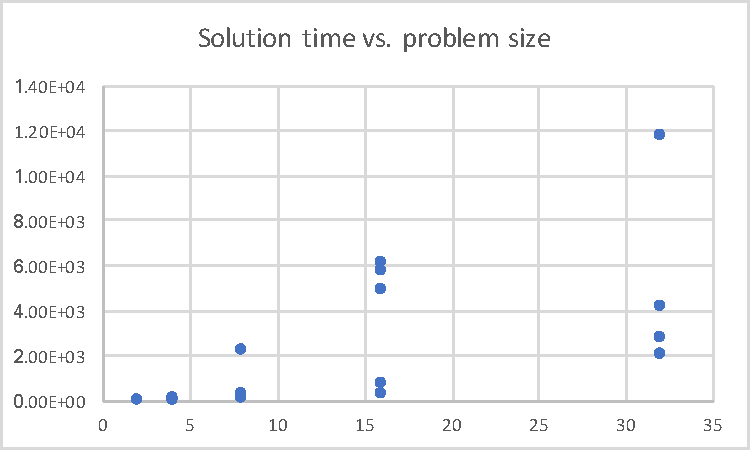
\includegraphics[width=\columnwidth]{graphics/ode_time_vs_problem_size.pdf}
\caption{Preliminary time to convergence vs. problem size.}
\end{figure}

The axes are the time to solution, plotted against $N$, the number of real numbers we are sorting.
The data points come from multiple random trials at each $N$.
The set of real numbers is randomly generated from a chosen dynamic range.
It appears that as the $N$ size increases, the average time grows linearly with respect to $N$.
Furthermore, the variance of the solution time, measured as the standard deviation, also grows.

\begin{figure}[h]
\centering
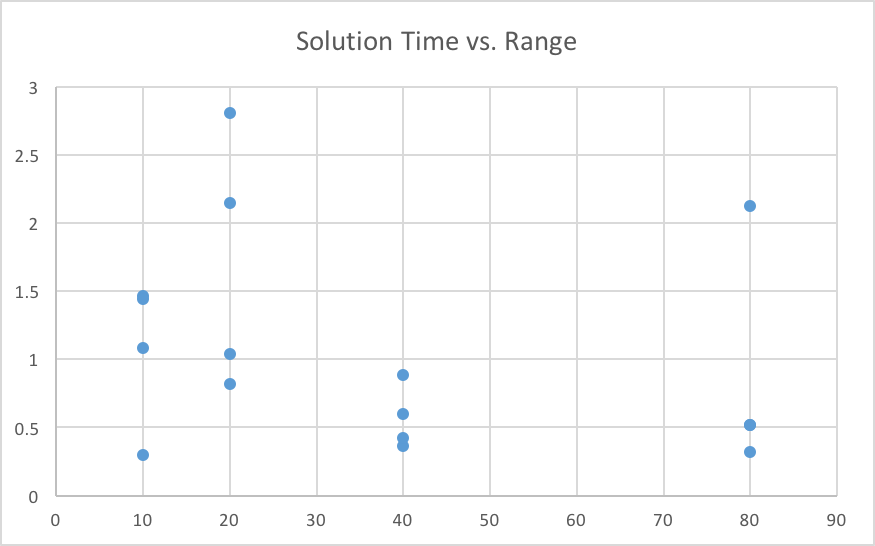
\includegraphics[width=\columnwidth]{graphics/range_vs_solution.png}
\caption{Preliminary time to convergence vs. dynamic range.}
\end{figure}

Another possible factor for solution time to consider is the dynamic range of the real numbers to sort. However, running the simulation on a constant number of elements with different dynamic ranges did not show any significant trends.

\subsection{Hardware cost of analog sorting}

Analog sorting on the chip relies on the hardware components needed to build the circuit. 
We need a constant amount of components for each of the $N$ ODEs.
Thus, the analog sorter takes up $O(N)$ amount of circuit components to sort $N$ elements.

\subsection{Limitations}

As mentioned before, the choice of initial $y$ values affects the sorting mechanism. Changing the initial values of the off-diagonals impacts whether or not the algorithm ever reaches a correctly sorted state of the diagonal entries.

Setting the initial values for the off-diagonals to $0$ will prevent the algorithm from starting in the first place. Initial $y$ values that are too small may stop the algorithm mid-way and result in an approximate sorting with two elements being out of place. After the diagonal entries converge to their final state, the $y$ values are nonzero, but in the magnitude of less than $10^{30}$. How big the initial off-diagonal entries have to be might depend on the range of the numbers to sort.

Brockett mentions briefly that $H_\infty$ will be sorted in almost all cases, but does not elaborate on the exceptions ~\cite{brockett}.


% \begin{figure}
% \centering
% \includegraphics[height=1in, width=1in]{fly}
% \caption{A sample black and white graphic
% that has been resized with the \texttt{includegraphics} command.}
% \end{figure}

% \begin{figure*}
% \centering
% \includegraphics{flies}
% \caption{A sample black and white graphic
% that needs to span two columns of text.}
% \end{figure*}

% \begin{figure}
% \centering
% \includegraphics[height=1in, width=1in]{rosette}
% \caption{A sample black and white graphic that has
% been resized with the \texttt{includegraphics} command.}
% \vskip -6pt
% \end{figure}

\section{Applications \& conclusions}
In this work, we validate that analog sorting works in practice.
While this idea has been presented several times in mathematical literature, this is the first where it is tested in practice, using analog computer hardware.
Using real measurements and simulated experiments, we evaluate the performance and efficiency of analog sorting.
We compare this technique against classical sorting algorithms.
In addition, we find limitations to analog sorting through experiments. Cases in which analog sorting could fail have not been discussed in previous literature.

In terms of concrete impact of our findings, analog sorting can be a new way to sort in future computer architectures.
Sorting is the underpinning of big data.
Increasingly, approximate sorts are useful.

In terms of the impact of this work on the future of analog computer techniques, we show in this paper two key ideas.
One, using the soliton behavior of the finite Toda lattice, we are able to swap two values in an analog computer without having to use a third capacitor as a buffer.
Two, it is possible to perform a typically ``discrete'' task using continuous-time hardware.
From this discrete primitive operation, we can build other discrete algorithms.


% What's exciting about this idea is it solves a deeply discrete problem using continuous methods.
% Furthermore, aside from this collection of references, the idea hasn't been explored elsewhere.

%ACKNOWLEDGMENTS are optional
\section{Acknowledgments}
This section is optional; it is a location for you
to acknowledge grants, funding, editing assistance and
what have you.  In the present case, for example, the
authors would like to thank Gerald Murray of ACM for
his help in codifying this \textit{Author's Guide}
and the \textbf{.cls} and \textbf{.tex} files that it describes.

%
% The following two commands are all you need in the
% initial runs of your .tex file to
% produce the bibliography for the citations in your paper.
\bibliographystyle{abbrv}
\bibliography{paper}  % sigproc.bib is the name of the Bibliography in this case
% You must have a proper ".bib" file
%  and remember to run:
% latex bibtex latex latex
% to resolve all references
%
% ACM needs 'a single self-contained file'!
%
%APPENDICES are optional
%\balancecolumns
\appendix
%Appendix A

\end{document}
